\documentclass[letterpaper,12pt]{article}

\usepackage{setspace}
\onehalfspacing

% waste less space around section titles etc.
\usepackage{titlesec}
\titlespacing*{\section}
{0pt}{1ex}{0.65ex}%{0pt}{1.5ex}{0.75ex}
\titlespacing*{\subsection}
{0pt}{0.9ex}{0.4ex}%{0pt}{1ex}{0.5ex}
\titlespacing*{\subsubsection}
{0pt}{0.7ex}{0ex}%{0pt}{0.75ex}{0ex}
\titlespacing*{\paragraph}
{0pt}{0.7ex}{1em}%{0pt}{0.75ex}{1em}

\usepackage[margin=1in]{geometry}
\usepackage{pdfpages}
\usepackage{microtype}
\usepackage{wrapfig}
\usepackage{subcaption}
\usepackage{amsmath,amssymb,amsthm}
\usepackage{hyperref}
\usepackage{array}
\usepackage{booktabs,url}
\usepackage{color}
\usepackage{afterpage}
\usepackage{enumitem}
\usepackage{times,psfrag,epsf,epsfig,graphics,graphicx}
\usepackage{algorithm}
\usepackage{algorithmic}
\usepackage{fancyvrb}
\usepackage{cite}

\usepackage{tikz}
\usetikzlibrary{arrows.meta}

%%%%%%%%%%%%%%%%% actual document starts here

\title{Truncating Blockchains with Tangly Statistics}

% change these to what applies
\author{Nathan Stouffer advised by Dr. Mike Wittie}
\date{}

\begin{document}

\maketitle

\begin{abstract}
    % blockchains are interesting and useful
    Blockchains provide a way to decentralize ledger-keeping systems.
    They are best known for their use in cryptocurrencies, but blockchains also have applications in supply chain tracking, providing data integrity, and any situation where immutable data is useful.
    To provide immutability, some blockchains use Proof of Work to construct an ever growing chain of blocks in a peer to peer network.
    Miners are expected to expend computational work to create a new block.
    Since blocks are intentionally difficult to create, users of a blockchain can trust the information held in the longest blockchain.

    % problem with blockchains
    Miners have collective control over a blockchain.
    If miners are sufficiently decentralized, then only a large coalition of miners could  gain explicit control of a blockchain.
    Explicit control allows the coalition to decide which blocks are added to the chain, reducing the integrity of the system.
    Thus a blockchain perform better when control of the chain is decentralized.
    Decentralized mining can be difficult to achieve when blockchains grow to an unmanageable length.
    To begin mining, one must download and process the entire chain.
    This is not a problem when the chain is relatively small, but a larger chain (such as Bitcoin) can take days to process.

    Excessively long chains limit decentralization in two ways.
    First, lightweight devices are prevented from becoming miners.
    Soon, many desktops and laptops will not be able to become a Bitcoin miner.
    Second, incredibly long bootstrapping time deters participation from users who do have sufficient space.
    Together, these issues decrease decentralization which reduces the effectiveness of a blockchain.

    % idea for a solution
    Over the summer, I worked with collaborators to devise a protocol that prunes blocks while preserving the chain's integrity.
    We ended the summer with a solution sketch that has potential but still needs significant work.
    At a high level, our solution has miners of recent blocks vote for a blockchain summary.
    If sufficiently many votes agree, bootstrapping nodes can trust the blockchain summary, which drastically reduces onboarding times.

    % implementation
    For my capstone project, I will extend the solution sketch from this summer.
    There are still issues to resolve and I must provide formal security proofs.
    Following this, I will implement a model of our solution.
    Using the model, I will run simulations and extract experimental results.
\end{abstract}


\section{Introduction}
\label{sec:introduction}

% >> This needs to tell a story: big picture problem, identify a "shortcoming", narrow it down to a specific gap that you are going to address.

% societal problem
% technical problem
% technical solution
% expected impact

Blockchain was introduced in order to provide distributed consensus without relying on a central party~\cite{nakamoto2009bitcoin}.
Avoiding a central party provides two benefits.
First, there is no central location that an attacker can access to compromise a system.
A centralized blockchain is much easier to compromise than a decentralized blockchain.
Second, there is no single party with complete control over a system.
An example of where decentralized control is useful is in international currency exchange.
Banks have the power to charge high transaction fees for international monetary transfers and customers are forced to pay the fees because there is no alternative.
Legitimate cryptocurrencies have enough competition between parties (miners) that there is no room for a monopoly, giving customers a cheaper option.

Bitcoin was released to the general public in 2009 as the first implementation of a blockchain.
Bitcoin garnered a lot of support and quickly became one of the most prominent cryptocurrencies.
Since Bitcoin's inception, blockchains have found other applications.
They are used in other cryptocurrencies, verify supply chains, and increase device autonomy in the Internet of Things~\cite{cai2018DecentralizedApplications}.
Blockchains are even being used to provide security and privacy in the medical field~\cite{siyal2019MedicalApplications}.
Blockchain technology has the potential to enhance data security in a wide range of diverse applications.

Blockchain’s services are best realized when control of the chain is decentralized.
Decentralized control can become difficult to achieve when blockchains grow to an unmanageable size.
I am writing this proposal to request funding to work on a method to truncate  blockchains.
My work on this project will be a continuation from the REU research I collaborated on this summer.
We have a solution sketch and a prototype implementation, but more work needs to be done to prove the correctness of the solution and to translate the prototype to a practical implementation.
If successful, this project has the possibility of making blockchains more effective, extending data reliability and user privacy~\cite{cai2018DecentralizedApplications}~\cite{siyal2019MedicalApplications}.

The remaining sections provide information regarding background information, my plan, an estimated time line, and other logistical details.


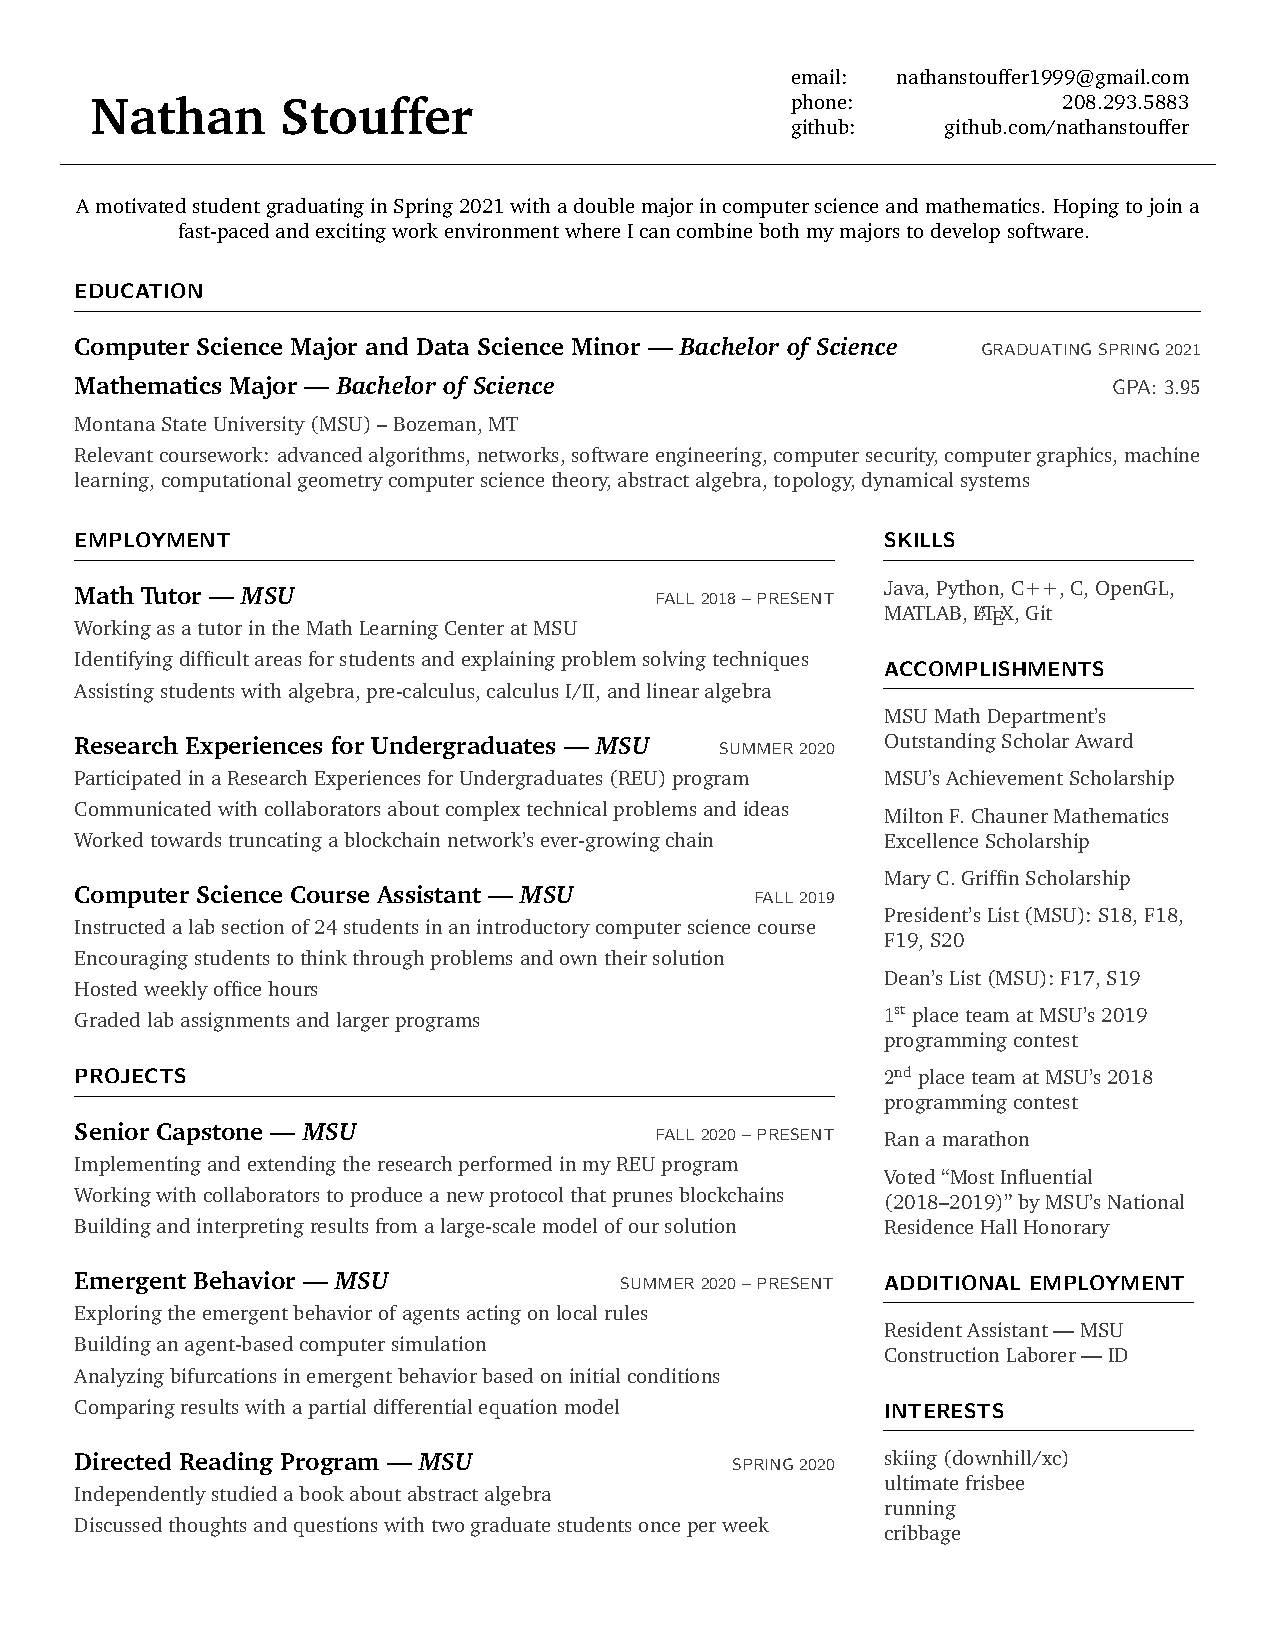
\includepdf[pages=-]{resume.pdf}

\section{Background}
\label{sec:background}

\subsection{Blockchain}

At a high level, a blockchain is a sequence of blocks that is immutable in practical applications.
Immutability in blockchains is often provided through Proof of Work.
Proof of Work was introduced in \cite{dwork1992PoW} and first used for blockchain in the Bitcoin whitepaper \cite{nakamoto2009Bitcoin}.
In a Proof of Work blockchain, a block is valid if its cryptographic hash is below a preset threshold.
The threshold is determined by the blockchain community.
It is typically set such that mining a block takes the same amount of time, on average, throughout the life of a blockchain.
The threshold will adapt as blocks are created to meet this requirement.
Each block primarily consists of data that cannot change (financial transactions, medical records, etc).
However, every block contains a field for a fixed-length string of arbitrary bits.
The fixed length string is called a nonce~\cite{nakamoto2009Bitcoin}.
``Mining'' a block consists of searching for a nonce that results in the hash of the block being below the threshold.
By design, it is difficult to find such a nonce because the hash function is cryptographic.
A miner's best strategy is to guess and check nonces until finding a sufficiently low output.
In cryptocurrencies, miners are awarded currency for their work.
Figure \ref{fig:blockchain} displays the typical structure of a blockchain.

\begin{center}
	\vspace{1em}
    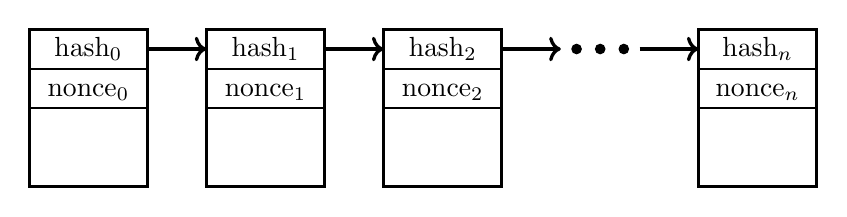
\begin{tikzpicture}
    % blockchain figure

    % boxes (w,l) = (1.5,2)
    \draw [very thick] (0,0) rectangle (1.5,2);
    \node at (0.75,1.75) {hash$_0$};
    \draw [thick] (0,1.5) -- (1.5,1.5);
    \node at (0.75,1.2) {nonce$_0$};
    \draw [thick] (0,1) -- (1.5,1);

    \draw [very thick] (2.25,0) rectangle (3.75,2);
    \node at (3,1.75) {hash$_1$};
    \draw [thick] (2.25,1.5) -- (3.75,1.5);
    \node at (3,1.2) {nonce$_1$};
    \draw [thick] (2.25,1) -- (3.75,1);

    \draw [very thick] (4.5,0) rectangle (6,2);
    \node at (5.25,1.75) {hash$_2$};
    \draw [thick] (4.5,1.5) -- (6,1.5);
    \node at (5.25,1.2) {nonce$_2$};
    \draw [thick] (4.5,1) -- (6,1);

    \draw [very thick] (8.5,0) rectangle (10,2);
    \node at (9.25,1.75) {hash$_n$};
    \draw [thick] (8.5,1.5) -- (10,1.5);
    \node at (9.25,1.2) {nonce$_n$};
    \draw [thick] (8.5,1) -- (10,1);

    % lines (length 0.75)
    \draw [->, very thick] (1.5,1.75) -- (2.25,1.75);
    \draw [->, very thick] (3.75,1.75) -- (4.5,1.75);
    \draw [->, very thick] (6,1.75) -- (6.75,1.75);
    \draw [->, very thick] (7.75,1.75) -- (8.5,1.75);

    % dots
    \draw [fill=black] (6.95,1.75) circle (0.06);
    \draw [fill=black] (7.25,1.75) circle (0.06);
    \draw [fill=black] (7.55,1.75) circle (0.06);

    \end{tikzpicture}
    \captionof{figure}{Prototypical Proof of Work Blockchain \label{fig:blockchain}}
\end{center}


A broader perspective of a blockchain is an implementation of a finite state machine.
In the state machine, blocks are transitions between the states of applications running on top of a blockchain.
Abstractly, the $k^{th}$ block $B_k$ is a transition from state $S_{k-1}$ to state $S_k$ with certain validity requirements.
See Figure \ref{fig:statemachine} for a visual.
A tangible example is a cryptocurrency.
Cryptocurrencies realize state as a record of the amount of currency each public key controls.
Blocks are a set of transactions that transfer currency between public keys (analogous to accounts).
In state $S_0$, no one controls any currency.
Then block $B_1$ is created and its miner is granted some currency.
This moves the blockchain to $S_1$ which records how much currency that miner controls.
Then block $B_2$ is mined, granting cryptocurrency to its miner.
Additionally, block $B_2$ could contain a currency transfer from the miner of the first block to another user.
Then the state $S_2$ records how much funds each user of the cryptocurreny controls.
Then block $B_3$ is created and the sate machine is updated with the changes in ``account'' balances.
This process repeats until state $S_n$ is reached, which contains the current account-balance pairs of all the current users of a cryptocurrency.

\begin{center}
    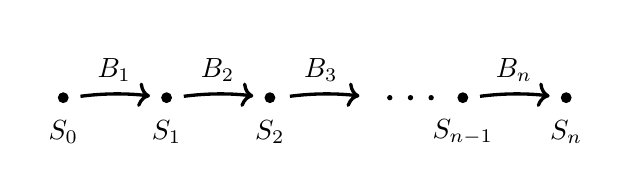
\begin{tikzpicture}[scale=1.75]
        % draw the 0 point
        \draw [thick,color=white] (0,0) -- (0,0);

        % state 0
        \draw [fill=black] (0.25,-0.5) circle (0.035);
        \node at (0.25,-0.75) {$S_0$};

        % block 1
        \draw [very thick, ->] (0.375,-0.49) arc (97.5:83:2);
        \node at (0.62,-0.3) {$B_1$};

        % state 1
        \draw [fill=black] (1,-0.5) circle (0.035);
        \node at (1,-0.75) {$S_1$};

        % block 2
        \draw [very thick, ->] (1.125,-0.49) arc (97.5:83:2);
        \node at (1.37,-0.3) {$B_2$};

        % state 2
        \draw [fill=black] (1.75,-0.5) circle (0.035);
        \node at (1.75,-0.75) {$S_2$};

        % block 3
        \draw [very thick, ->] (1.895,-0.49) arc (97.5:83:2);
        \node at (2.12,-0.3) {$B_3$};

        % ...
        \draw [fill=black] (2.62,-0.5) circle (0.015);
        \draw [fill=black] (2.77,-0.5) circle (0.015);
        \draw [fill=black] (2.92,-0.5) circle (0.015);

        % state n-1
        \draw [fill=black] (3.15,-0.5) circle (0.035);
        \node at (3.15,-0.75) {$S_{n-1}$};

        % block n
        \draw [very thick, ->] (3.275,-0.49) arc (97.5:83:2);
        \node at (3.52,-0.3) {$B_n$};

        % state n
        \draw [fill=black] (3.90,-0.5) circle (0.035);
        \node at (3.90,-0.75) {$S_n$};

    \end{tikzpicture}
    \captionof{figure}{Blocks as transitions between states \label{fig:statemachine}}
\end{center}


\subsection{Technical Problem}

To understand the technical problem, we must understand two properties of blockchains.
First, miners must obtain every block before mining new blocks.
And, second, blockchains grow in perpetuity.
These properties mean that new miners must download and process an ever increasing amount of data as time passes.
Even now, when Bitcoin is just over a decade old, it can take days to become a miner. % maybe cite Bernardini but they have no source for that claim
Such a barrier can deter large machines from the joining the chain and entirely prevent small machines from mining.

The root of the problem is that mining requires all the information in a blockchain.
Our goal is to produce an off-chain, efficient, and secure method to bootstrap miners in a blockchain.
An off-chain solution is one that does affect the underlying blockchain.
This is important because many on-chain solutions to this problem cause a hard fork in a blockchain.
A hard fork is when a blockchain splits because miners disagree on the format of a block~\cite{lin2017Survey}.
While a blockchain can survive a hard fork, the mining power splits and weakens the blockchain.
We want an efficient solution so that our idea could be useful in an actual blockchain.
Finally, security is important because blockchains often record important information such as medical records. 
Our solution should not introduce vulnerabilities to such important information.

To frame this project, we use the Goal Question Metric approach presented in \cite{basili1994goal}.
This results in ``the specification of a measurement system targeting a particular set of issues and a set of rules for the interpretation of the measurement data \cite{basili1994goal}.''
The model has three levels.
At the conceptual level, a goal is defined.
A goal consists of a purpose, an issue, a process, and a viewpoint.
At the operational level, a set of questions are asked that characterizes the goal.
At the quantitative level, data is associated with questions in an attempt to answer them.
The data can be either objective or subjective.
Table \ref{tab:gqm} displays the Goal Question Metric Approach we will use for this project.

\newpage 

\begin{table}[h]
    \centering
    \begin{tabular}{|ll|l|}
        \hline
        Goal & Purpose    & Decrease \\
             & Issue      & required time and space \\
             & Process    & bootstrap a node to a blockchain network \\
             & Viewpoint  & the bootstrapping node \\ \hline

        Question & Q1 & Is the solution off-chain? \\ \hline
        Metrics  & M1 & Number of changes to blockchain protocol (must be 0) \\ \hline

        Question & Q2 & Is the solution efficient? \\ \hline
        Metrics  & M2 & Asymptotic analysis of time and space requirements as the chain grows \\
                 & M3 & Bytes of network traffic generated \\ \hline

        Question & Q3 & Is the solution secure? \\ \hline
        Metrics  & M4 & Theoretical probability that a malicious actor fools a bootstrapping node \\
                 & M5 & Empirical probability that a malicious actor fools a bootstrapping node \\
        \hline
    \end{tabular}
    \caption{The Goal Question Metric approach for this project}
    \label{tab:gqm}
\end{table}


\subsection{Related Work}

Truncating the required bootstrapping information in a blockchain is an active area of research.
The remainder of Section \ref{sec:background} is devoted to summarizing existing ideas and solutions.

% lightweight nodes in the bitcoin whitepaper

The Bitcoin whitepaper~\cite{nakamoto2009Bitcoin} introduces the concept of lightweight nodes.
Instead of becoming a full node, lightweight nodes only store the header chain and query full nodes to see if transactions are valid.
This is a step in the right direction because the header chain downloads quickly, but it does not grant nodes the ability to mine new blocks.
Nodes can only verify old transactions.

% summary block in the main chain

Another idea is to periodically place a summary block in the original blockchain~\cite{palai2018BlockSummariesSameChain}~\cite{nadiya2018BlockSummaries(ExtendsPalai)}.
A summary block is responsible for reporting the net change caused by a certain amount of previous blocks.
This process can be made recursive to any depth by creating a summary block responsible for a set of summary blocks (a summary of summaries)~\cite{palai2018BlockSummariesSameChain}~\cite{nadiya2018BlockSummaries(ExtendsPalai)}.
Trust in the summary blocks is built in the same fashion as trust in the regular blockchain.
A node joining the network would download the header chain and relevant summary blocks.
If a summary block has been accounted for by another summary block, there is no need to download it.
This idea is nice because it relies on the same security principles as blockchain, but the implementation would require a hard fork.

% miniblockchain

A different idea would be to use mini-blockchain~\cite{bruce2014Miniblockchain}.
A mini-blockchain requires that a block $B_k$ includes the hash of $S_k$, cryptographically tying the state to the blockchain.
A bootstrapping node can then request the header chain, a recent state, and blocks following the recent state.
The new node can verify that the received state corresponds with the blockchain and then compute the current state with the information in the newest blocks.
While this solution is quite clean, it would cause a hard fork.

% separate summary chain

Another way to provide state would be to create a new blockchain that records state~\cite{marsalek2019BockSummariesSeparateChain}.
The new blockchain records the state of the original chain every so often and bootstrapping nodes can eliminate the need for blocks prior to the most recent summary.
Since each state exists independently of all other states, the size of the second blockchain will not bloat like the original chain~\cite{marsalek2019BockSummariesSeparateChain}.
While this solution does operate off-chain, it is not necessarily secure.
It is unlikely that a miner will give up valuable computing power to contribute to the second blockchain.
This could allow a powerful, malicious actor to sabotage the second blockchain, making it unreliable.

% coinprune

The final related idea holds an election to verify state~\cite{matzutt2020HowTSPrune}.
Miners are allowed to vote for a state and then bootstrapping nodes trust the majority of votes.
Each vote is recorded in a block and each block has the capacity to store a single vote~\cite{matzutt2020HowTSPrune}.
Storing votes in blocks makes them immutable, so a bootstrapping node is able to collect every vote.
The issues with this idea are two-fold.
First, a vote can only be generated as quickly as new blocks.
In Bitcoin, this averages to about 10 minutes per block~\cite{nakamoto2009Bitcoin}, meaning a bootstrapping node might have to wait a week for there to be sufficiently many votes to trust a state.
Second, \cite{matzutt2020HowTSPrune} relies on implementation details in the Bitcoin protocol and does not apply to blockchains in general.


\section{Solution}
\label{sec:solution}

\subsection{Idea}

Recall that our goal is to devise an off-chain, efficient, and secure bootstrapping method.
The primary barrier to this goal is that blockchains require that a miner to obtain every block in the chain.
Viewing blockchain as a finite state machine allows us to reduce the amount of information that a bootstrapping miner must obtain.
To compute the current state $S_n$, one need only know is some state $S_k$ and every block $B_j$ with $j > k$.
In standard blockchains, $S_k$ is $S_0$ and the bootstrapping node needs every block in the chain.
If $S_k$ is close to the end of the chain, then the miner only needs the blocks following $S_k$, which will download much faster!

At this point we have reduced the problem of bootstrapping to providing some recent state $S_k$ of the blockchain.
How does a bootstrapping miner obtain the state $S_k$?
They can't just ask a blockchain node, because the node might lie and give a false state.
To solve this, we draw from \cite{matzutt2020HowTSPrune} and host an election at regular intervals (say every 1000 blocks).
We allow recent miners to vote.
Note that miners are identified by the public keys in the blocks they mined, preventing identity theft.
If the election is for state $S_k$, then a miner computes the hash of their version of $S_k$.
The miner submits a digital signature of the hash; the signature should use the private key from the block the miner created.
The digital signature prevents a malicious actor from forging the vote.

The election is decided based on the relative vote distribution.
Let $V$ denote the total number of voters (not the number of votes cast).
For a tuneable $\beta \in (0.5,1]$, we will decide an election if greater than $\lceil \beta V \rceil$ votes agree.
However, we do not have every vote since voting is not required and votes can be deleted by malicious actors.
Instead, we have a sample of votes.
How can we figure out whether the sample was drawn from the required distribution?
The $\chi ^2$ goodness of fit test is a way to measure the probability that a sample comes from an expected distribution.
If the probability returned from the $\chi ^2$ test is above a tuneable threshold $\alpha$, we accept the state with the most votes.

The votes are submitted to a Distributed Hash Table (DHT).
Storing votes in a DHT is a compromise: it is convenient because miners can vote at their leisure, but a powerful, malicious actor can delete votes.
To combat vote deletion, we draw on the idea of a tangle \cite{popov2016Tangle}.
A tangle is a directed acyclic graph where the vertices are added to tangle by selecting the two most recently added vertices as parents.
In this context, vertices are realized as votes.

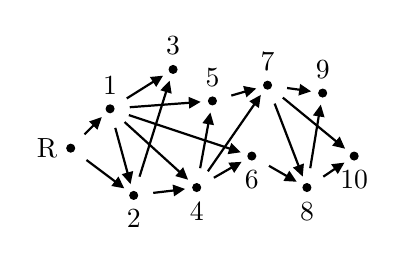
\begin{tikzpicture}[scale=2,rotate=270]
    %% vertices
    \draw [fill=black] (0.0,0.0)     circle (0.025);
    \draw [fill=black] (-0.25,0.25)  circle (0.025);
    \draw [fill=black] (0.3,0.4)     circle (0.025);
    \draw [fill=black] (-0.5,0.65)   circle (0.025);
    \draw [fill=black] (0.25,0.8)    circle (0.025);
    \draw [fill=black] (-0.3,0.9)    circle (0.025);
    \draw [fill=black] (0.05,1.15)   circle (0.025);
    \draw [fill=black] (-0.4,1.25)   circle (0.025);
    \draw [fill=black] (0.25,1.5)    circle (0.025);
    \draw [fill=black] (-0.35,1.6)   circle (0.025);
    \draw [fill=black] (0.05,1.8)    circle (0.025);
    %% labels
    \node at (0.0,-0.15) {R};
    \node at (-0.4,0.25) {1};
    \node at (0.45,0.4) {2};
    \node at (-0.65,0.65) {3};
    \node at (0.4,0.8) {4};
    \node at (-0.45,0.9) {5};
    \node at (0.2,1.15) {6};
    \node at (-0.55,1.25) {7};
    \node at (0.4,1.5) {8};
    \node at (-0.5,1.6) {9};
    \node at (0.2,1.8) {10};
    %% edges
    \draw [thick] (-0.088,0.088) -- (-0.162,0.162);
    \draw [thick] (0.075,0.1) -- (0.225,0.3);
    \draw [thick] (-0.129,0.283) -- (0.179,0.367);
    \draw [thick] (-0.316,0.356) -- (-0.434,0.544);
    \draw [thick] (-0.166,0.342) -- (0.166,0.708);
    \draw [thick] (-0.26,0.375) -- (-0.29,0.775);
    \draw [thick] (-0.21,0.369) -- (0.01,1.031);
    \draw [thick] (0.181,0.437) -- (-0.381,0.613);
    \draw [thick] (0.284,0.524) -- (0.266,0.676);
    \draw [thick] (0.127,0.822) -- (-0.177,0.878);
    \draw [thick] (0.188,0.909) -- (0.112,1.041);
    \draw [thick] (0.147,0.871) -- (-0.297,1.179);
    \draw [thick] (-0.334,1.02) -- (-0.366,1.13);
    \draw [thick] (0.112,1.259) -- (0.188,1.391);
    \draw [thick] (-0.283,1.295) -- (0.133,1.455);
    \draw [thick] (-0.382,1.374) -- (-0.368,1.476);
    \draw [thick] (-0.321,1.347) -- (-0.029,1.703);
    \draw [thick] (0.127,1.521) -- (-0.227,1.579);
    \draw [thick] (0.181,1.604) -- (0.119,1.696);
    %% arrows
    \fill [black] (-0.197,0.197) -- (-0.117,0.17) -- (-0.17,0.117);
    \fill [black] (0.255,0.34) -- (0.24,0.258) -- (0.18,0.303);
    \fill [black] (0.228,0.38) -- (0.165,0.324) -- (0.145,0.397);
    \fill [black] (-0.46,0.586) -- (-0.389,0.543) -- (-0.452,0.503);
    \fill [black] (0.2,0.745) -- (0.177,0.664) -- (0.121,0.714);
    \fill [black] (-0.294,0.825) -- (-0.251,0.753) -- (-0.326,0.748);
    \fill [black] (0.026,1.079) -- (0.038,0.996) -- (-0.033,1.02);
    \fill [black] (-0.428,0.628) -- (-0.346,0.641) -- (-0.368,0.569);
    \fill [black] (0.259,0.726) -- (0.306,0.656) -- (0.231,0.647);
    \fill [black] (-0.226,0.887) -- (-0.146,0.91) -- (-0.159,0.836);
    \fill [black] (0.087,1.085) -- (0.157,1.038) -- (0.092,1.001);
    \fill [black] (-0.338,1.207) -- (-0.255,1.195) -- (-0.298,1.134);
    \fill [black] (-0.379,1.178) -- (-0.323,1.116) -- (-0.395,1.095);
    \fill [black] (0.213,1.435) -- (0.208,1.351) -- (0.143,1.388);
    \fill [black] (0.18,1.473) -- (0.123,1.411) -- (0.097,1.481);
    \fill [black] (-0.361,1.526) -- (-0.334,1.446) -- (-0.408,1.457);
    \fill [black] (0.003,1.742) -- (-0.016,1.66) -- (-0.074,1.708);
    \fill [black] (-0.276,1.588) -- (-0.196,1.612) -- (-0.208,1.538);
    \fill [black] (0.092,1.738) -- (0.164,1.696) -- (0.102,1.654);
\end{tikzpicture}

A set of DHT nodes are designated as tangle managers, each given complete control of their own tangle.
A voter is expected to submit their vote to a deterministic subset of the tangles.
A tangle manager receives votes and inserts each of them to their tangle by attaching them to parent votes.
If a vote is not in every tangle of the deterministic subset, then it is considered invalid.
The children of an invalid vote are also invalid.
Then, deleting a vote causes a chain reaction that invalidates all the descendant of the deleted vote.
The distribution of states that the descendants support matches the distribution of cast votes, so a malicious actor cannot swing an election by selectively deleting votes.
A bootstrapping node can request the vote tangles and then make a decision based on valid votes.

\subsection{Implementation}

This capstone project will include a model implementation of the solution.
The implementation will run a full-fledged DHT running on top of a network simulator.
Scripted miners will submit votes to the DHT and bootstrapping nodes will request the tangles and decide the election.
Using the simulation, we can gather empirical results indicating the security of our solution.
The network simulator will allow us to gather information about the amount of network traffic required to facilitate an election.

\section{Methodology}
\label{sec:methodology}

% provide enough information so that someone can replicate

Much of this project is devising a method to bootstrap blockchain nodes.
Since this is a conceptual task, it cannot be replicated.
However, the experimental verification of our protocol can be replicated.
Section \ref{sec:methodology} is devoted to providing the necessary information for someone to replicate our implementation.

% network simulator with dht

In order to match our model as closely as possible with our implementation, we chose to implement our solution on a network simulator using a full-fledged DHT.
This is not strictly necessary but we felt that it made our results more applicable to a real implementation of our idea.

% digitally signed parents

A neglected detail of the solution is the process of selecting parents in the tangle.
The tangle manager has complete control over \textit{which} votes are selected as parents, but we require that the parents are digitally signed in the vote.
This means that the manager must tell the voter which votes are the parents and the voter includes that information in their vote.
While this is some overhead communication for our solution, it prevents a malicious actor from changing the structure of a tangle to their advantage.

% attacker intelligence

The most important aspect of the implementation is the intelligence of the attackers.
We expect the constraints of our solution to prevent an attacker from \textit{successfully} fooling a bootstrapping node.
But the only way we can verify this is to simulate intelligent attackers.
We have divided attacks into three categories: creating votes, deleting votes, and reordering votes.
An accurate replication of this project should at least implement these strategies.
Implementing more strategies is welcome, since it provides more information on our system!

% chi-squared test

We used the $\chi ^2$ test as follows.
Consider some sample of votes $S$ and our expected proportion of agreeing votes $\beta$.
Our distribution comes in the form $(majority, other)$ where $majority$ references the number of valid votes that supported the most popular state and $other$ is the number of valid votes that did not support the most popular state.
We have an expected distribution $(\beta|S|, (1-\beta)|S|)$ and an actual distribution of $(S_{maj}, S_{oth})$.
Then we can use the $\chi ^2$ test to determine the probability that our sample comes from the expected distribution.

\subsection{Design}

The design pattern that appears in this project is the Strategy Pattern.
The design pattern presents itself in the different attack styles that we will simulate: creating votes, deleting votes, and reordering votes.
We will have an adversary interface with a method callled \textit{attack()}.
Each class that implements an attack type will implement that interface.
Figure \ref{fig:strategy} shows a visual of our Unified Modeling Language diagram for this pattern.

\newcommand{\operation}{$+$\textit{sortedVotes()} : String[]}

\begin{center}
	\vspace{1em}
    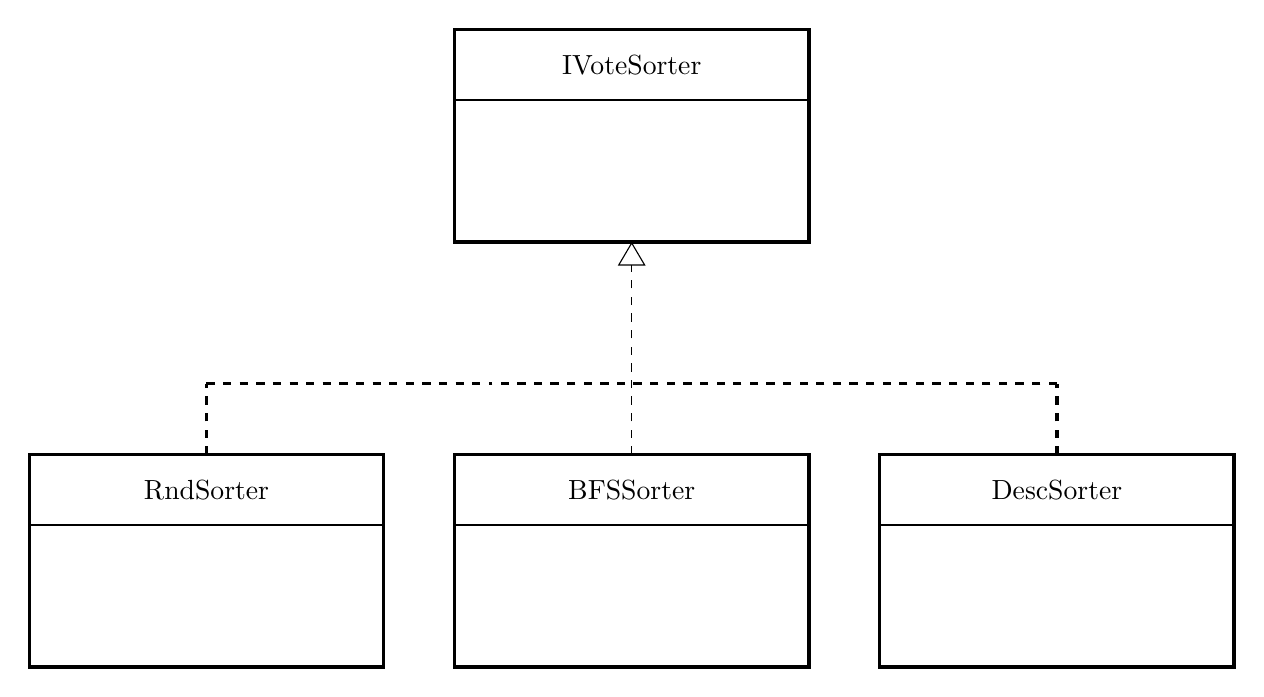
\begin{tikzpicture}[scale=0.9]
    % uml figure

    % boxes (w,l) = (5,3)
    \draw [very thick] (6,6) rectangle (11,9);
    \node at (8.5,8.5) {IVoteSorter};
    \draw [thick] (6,8) -- (11,8);
    \node at (8.5,7.65) {\operation};

    \draw [very thick] (0,0) rectangle (5,3);
    \node at (2.5,2.5) {RndSorter};
    \draw [thick] (0,2) -- (5,2);
    \node at (2.5,1.65) {\operation};

    \draw [very thick] (6,0) rectangle (11,3);
    \node at (8.5,2.5) {BFSSorter};
    \draw [thick] (6,2) -- (11,2);
    \node at (8.5,1.65) {\operation};

    \draw [very thick] (12,0) rectangle (17,3);
    \node at (14.5,2.5) {DescSorter};
    \draw [thick] (12,2) -- (17,2);
    \node at (14.5,1.65) {\operation};

    % lines
    \draw [dashed, -{Triangle[open, width=3.5mm, length=3mm]}] (8.5,3) to (8.5,6);
    %\draw [dashed, very thick] (6.5,3) -- (6.5,5.7);
    \draw [dashed, very thick] (2.5,3) -- (2.5,4);
    \draw [dashed, very thick] (2.5,4) -- (6.5,4);
    \draw [dashed, very thick] (14.5,3) -- (14.5,4);
    \draw [dashed, very thick] (14.5,4) -- (6.5,4);

    \end{tikzpicture}
    \captionof{figure}{Strategy Pattern for vote sorters\label{fig:strategy}}
\end{center}



\section{Results}
\label{sec:results}

% this section must be devoid of opinion

\begin{figure}[h]
	\centering
	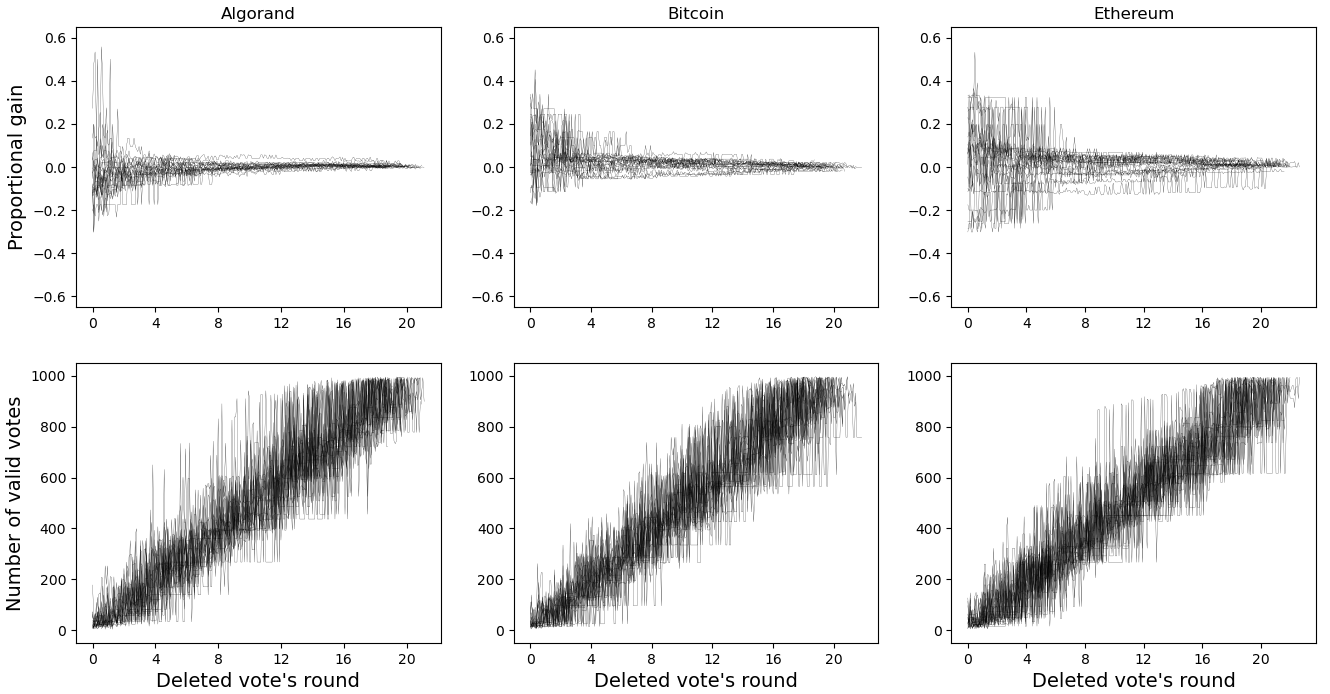
\includegraphics[width=\linewidth]{img/deleter}
	\caption{INSERT CAPTION}
	\label{fig:deleter}
\end{figure}

\begin{figure}[h]
	\centering
	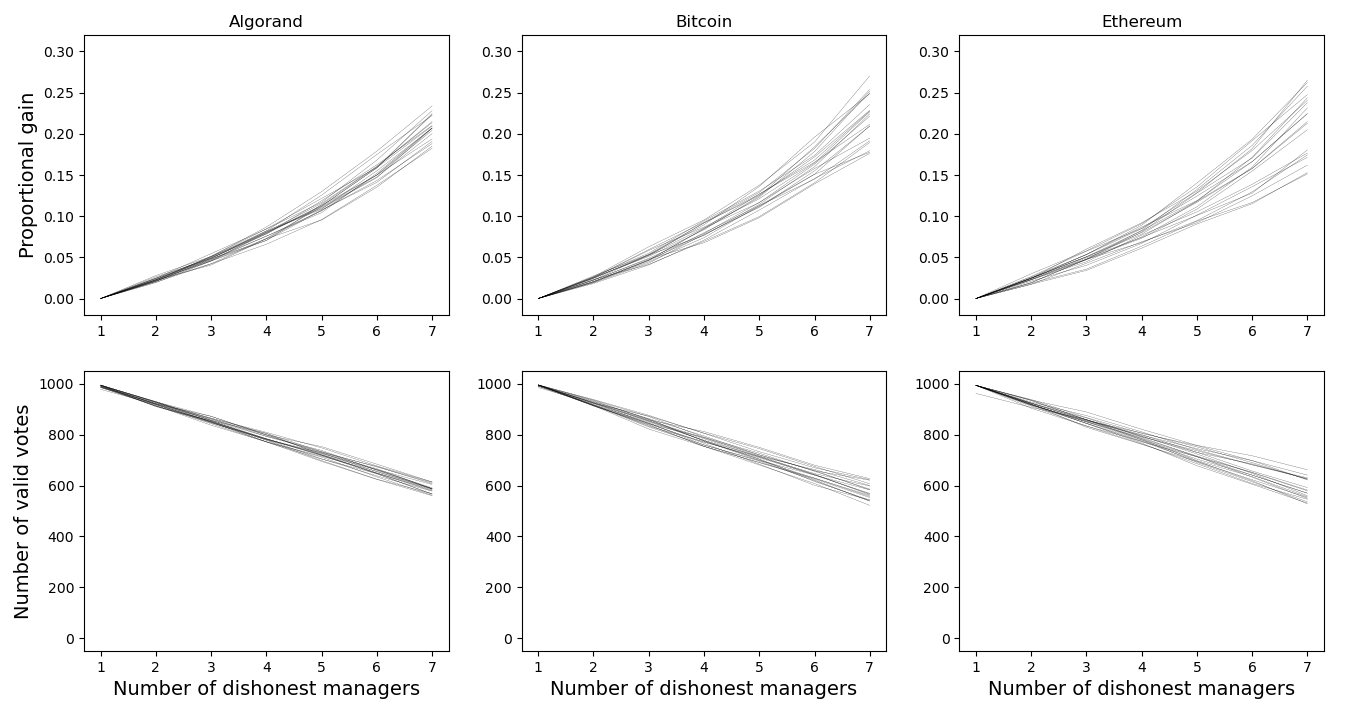
\includegraphics[width=\linewidth]{img/rejecter}
	\caption{INSERT CAPTION}
	\label{fig:rejecter}
\end{figure}

\section{Discussion}
\label{sec:discussion}

\section{Conclusion}
\label{sec:conclusion}

% conclude and discuss future work

%%%%%%%%%%%%%%%

\clearpage

\bibliographystyle{unsrt}
\bibliography{bibliography/refs}

\clearpage

\end{document}
